\chapter{General Introduction}
%\addstarredchapter{General Introduction}
%-------------------------------------------------------------------------------------------------------------------------------------------------
Casting is one the earliest production techniques created by human civilisation since the Bronze Age, dated to circa 3000 BC. 
From ancient swords to nowadays toys, the need for alloys has never decreased.
The key phenomenon behind this technique is solidification, or the transformation of matter from liquid to solid state. With this phase change, 
many phenomena, not visible to the naked eye, take place with a very complex interaction, in order to form a solid. 
However, the combination of thermal phenomena, like release of latent heat of solidification, and chemical phenomena like redistribution of chemical
element atoms (also known as solute) with other atoms, often lead to \emph{segregation}. The origins of this
word from Latin, \emph{segregatus}, has a social meaning of "separating a group from the dominant majority", while 
in metallurgy it means a non uniform distribution of chemical species. Depending on the scale, we may speak of \emph{microsegregation}
when the heterogeneity spans some few hundred microns, whereas the term \emph{macrosegregation} refers to a much coarser length scale, ranging
from some millimetres to some meters! The final solid structure is has intrinsic thermophysical and thermomechanical properties directly influenced by the segregation pattern. 
In casting processes, such as continuous casting (\cref{fig:casting}) and ingot casting, it is crucial to apprehend 
these intricate phenomena leading to macrosegregation as well as the influence on the final product, at each step of the process. 

In this introductory chapter, we give a quick overview of solidification phenomena and microstructure, then present the factors which
promote segregation, on both microscopic and macroscopic scales. Aside from macrosegregation, others defects are also briefly presented.
%-----------------
\begin{figure}[htbp]
\centering
   %------------
  \begin{subfigure}[t]{0.6\textwidth}
    \centering
	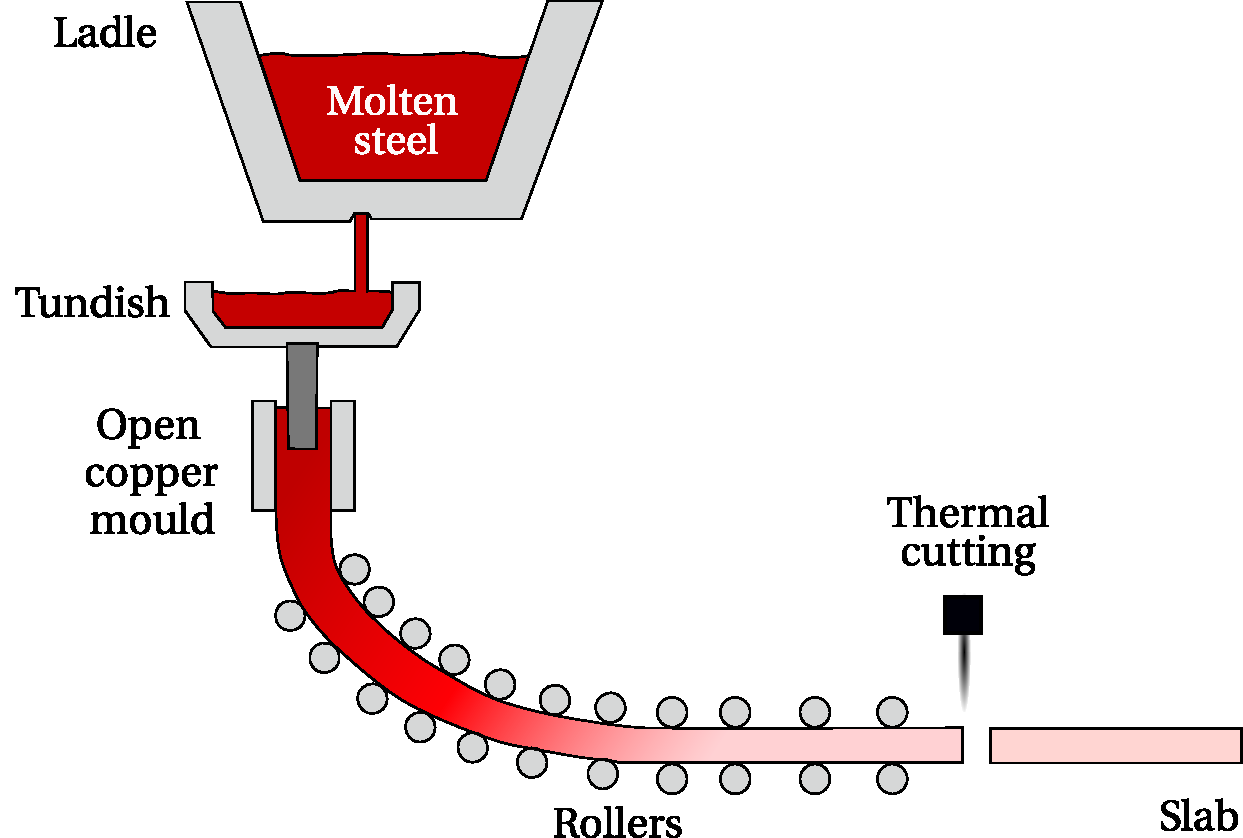
\includegraphics[height=5cm]{Chapter1/Graphics/fig_continuous_casting.pdf}
	\caption{}
    \label{fig:continuous_casting}
  \end{subfigure}
   %------------
   %\hspace{1cm}
   \begin{subfigure}[t]{0.3\textwidth}
    \centering
	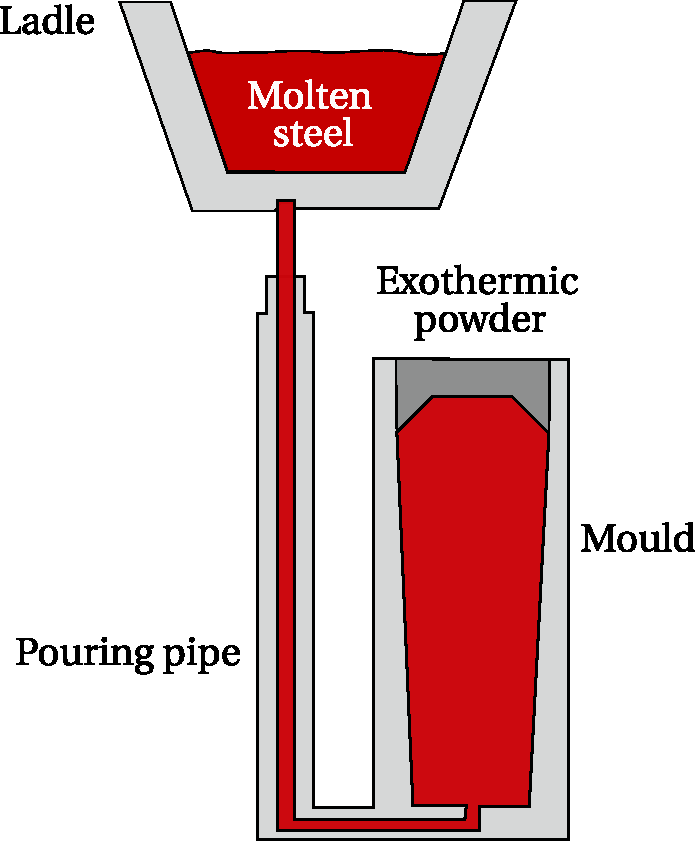
\includegraphics[height=5cm]{Chapter1/Graphics/fig_ingot_casting.pdf}
	\caption{}
    \label{fig:ingot_casting}
  \end{subfigure}
\caption{Main steelmaking processes by (a) continuous casting or (b) ingot casting} 
\label{fig:casting}
\end{figure}
%
%-------------------------------------------------------------------------------------------------------------------------------------------------
%
In a continuous casting process (\cref{fig:continuous_casting}), the partially solidified slab is carried through a series of rolls that exert contact forces to straighten it.
As the mushy part of a slab enters through these rolls, interdendritic liquid is expelled backwards, i.e. in regions with lower solid fraction.
Since the slab edges solidify earlier than the centre, the enriched liquid accumulates halfway in thickness, forming a centreline macrosegregation
as shown in \cref{fig:macroseg_centreline}. Other types of segregates (channels, A-segregates ...) can also be found but remain more specific to ingot casting. 
A variety of segregation patterns can be encountered while casting heavy ingots, as in \cref{fig:ingot_casting}: 
\begin{itemize}
\itemsep0em 
\item the lower part is characterized by a negative segregation cone promoted by the sedimentation of 
	  equiaxed crystals and settling of dendrite fragments,
\item positive segregation channels, known as A-segregates, form along the columnar dendritic zones, close to the vertical contact with the mould,
\item positive V-segregates can be identified in the centre of the ingot,
\item a positive "hot-top" macrosegregation in the upper zone where the last rich liquid solidifies, caused by solidification shrinkage and thermosolutal buoyancy forces. 
\end{itemize}
\citet{combeau_prediction_2009} state that A-segregates and V-segregates formation is mainly attributed to local flow phenomena.
As such, their scale is finer than macrosegregation, hence called "mesosegregates".
%--------------
\begin{figureth}
% macrosegregation_centreline_zoom: http://goo.gl/iKPNfz
% textwidth 
{1.0}
%path 
{Chapter1/Graphics/macrosegregation_centreline_zoom.pdf}
% caption
{Zoom on a sulphur print of a continuously cast high carbon steel billet at a longitudinal section, showing high positive centreline segregation \citep{choudhary_morphology_2007}.}
% label
\label{fig:macroseg_centreline}
\end{figureth}
%--------------
%--------------------------------------------------------
%
%-----------------------
\begin{figureth}
{1.0}
{Chapter1/Graphics/macrosegregation_ingot.png}
{Sulphur print (left) of a 65-ton steel ingot \citep{lesoult_macrosegregation_2005} showing various patterns (right) of macrosegregation \citep{flemings_solidification_1974}}
\label{macrosegregation_ingot}
\end{figureth}
%--------------------------------------------------------
%
%***********************************************
\section{Solidification notions}
%***********************************************
%
%***********************************************
\subsection{Solute partitioning}
%***********************************************
The simplest definition is of this phenomenon is an uneven distribution of solute between the liquid and the growing solid, at the microscopic scale
of the interface separating these phases. If we consider a binary alloy, then the solubility limit is 
the key factor that dictates the composition at which a primary solid phase exists at equilibrium. 
The segregation (or partition) coefficient $\k$ determines the extent of solute rejection into the liquid during solidification:
%----------------------
\begin{align}
\label{eq:partition}
& \k = \frac{\Csstar}{\Clstar}
\end{align}
%----------------------
where $\Csstar$ and $\Clstar$ are the compositions of the solid and liquid respectively, at the interface. When the 
segregation coefficient is less than unity (such is the case for most alloys during dendritic solidification), 
the first solid forms at the liquidus temperature, $T$, with a composition $\Csstar=\k \Clstar=\k \Cnominal$ less than the liquid's 
composition $\Cnominal$, the latter being initially at the nominal composition, $\Cnominal$. \Cref{fig:binary_diag} illustrates a typical binary 
phase diagram where the real solidus and liquidus are represented by solid lines, while the possible linear approximations are in grey dashed lines.
For most binary alloys, this linearisation simplifies derivation of microsegregation models, as $\k$ becomes independent of temperature.

For each phase, the relationship between the composition at the interface and that in the bulk depends on the chemical homogenisation (i.e. solute diffusivity) of the phase.
The more homogeneous a phase, the closer the concentrations between the interface and the bulk, hence closer to equilibrium.
%The higher the diffusion coefficient of the phase, $\Dphi$, the closer the concentrations between the interface and the bulk. 
It is thus essential to study the effect of homogenisation on the segregation behaviour and the subsequent effect on solidification, 
which is seen by a non-uniform composition through the cast product on a microscopic scale, better known as microsegregation.
This phenomenon is essential in a casting process inasmuch as it affects the microstructure and grain morphology, hence the final
mechanical properties of the alloy.
%----------------------
\begin{figureth}
% textwidth 
{0.5}
%path 
{Chapter1/Graphics/PhaseDiagram.pdf}
% caption
{Typical eutectic phase diagram of a binary alloy showing the real solidus and liquidus at full equilibrium,
with the corresponding linear approximations (grey dashed lines). $T_m$ and $T_E$ are respectively the melting point
of the solvent and the eutectic temperature.}
% label
\label{fig:binary_diag}
\end{figureth}
%
%***********************************************
\subsection{Dendritic growth}
%***********************************************
In a casting process, the chill surface i.e. the contact between the molten alloy and relatively cold moulds, is the first area to solidify. 
Thermal gradient, $G$, and cooling rate, $R$, are two crucial process parameters that define the solid-liquid interface velocity, $\vstar$, which in turn
affects the initial microstructure. Although it may be not easy to control them, their crucial role in solidification is well established.

The solid-liquid interface fluctuates when solidifying, thus perturbations may appear on the front, locally destabilizing it. 
Two outcome scenarios are possible.
%----------------------
\begin{figureth}
% textwidth 
{1.0}
%path 
{Chapter1/Graphics/dendrite_evolution.pdf}
% caption
{Time evolution of a solidifying \bin{Al}{4}{Cu} sample, showing interface destabilisation and subsequent dendritic solidification \citep{buffet_measurement_2010}.
The liquid far from the interface and having a blue color is at nominal composition, while the one near the dendritic structure with the yellow and red colors, is richer in solute.}
% label
\label{fig:dendrite_evolution}
\end{figureth}
%-----------------------------------
%
The first scenario is characterized by low values of $\vstar$ where the interface maintains a planar shape, hence we speak of \emph{planar growth}. 
With this kind of growth, a random protuberance appearing at the interface, has a low tip velocity (low driving force of solidification). As such,
the rest of the interface catches up, maintaining the planar geometry.
In another scenario more representative of a real casting, the interface speed is greater in general, due to high solidification rate.
The protuberance tip will be pulled into a liquid less rich in solute than the interface, as shown in the time frames of \cref{fig:dendrite_evolution}.
The zone ahead of the solid-liquid interface is constitutionally undercooled \citep{tiller_redistribution_1953}, 
giving a greater driving force for the protuberance to grow in the direction
of the thermal gradient. As the solid-liquid interface adopts a tree-like shape, we speak of \emph{dendritic growth}. Near the chill surface, dendrites are columnar, with a 
favourable growth in the <100> direction for alloys with cubic lattices, but different orientations are also reported in the literature \citep[see][289]{dantzig_solidification_2009}.
Far from mould walls, a similar dendritic growth phenomenon occurs where temperature is uniform, but with an equiaxed morphology.
\Cref{fig:dendritic_growth} shows both columnar and equiaxed morphologies. Columnar dendrites are characterised by a primary spacing, 
$\pdas$, between the main trunks, and a secondary spacing, $\sdas$, for the arms that are perpendicular
to the trunks. It should be noted that $\pdas$ and $\sdas$, together with the grain size, are three important 
microstructural parameters in the as-cast microstructure \citep{easton_grain_2011}.
Further branching may occur but will not be discussed here.
%-----------------
\begin{figure}[htbp]
\centering
   %------------
  \begin{subfigure}[t]{0.45\textwidth}
    \centering
	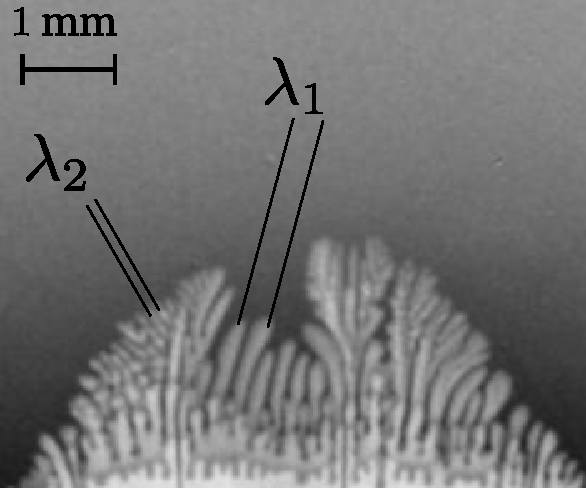
\includegraphics[height=4cm]{Chapter1/Graphics/dendrite_C.pdf}
	\caption{}
    \label{fig:dendrite_C}
  \end{subfigure}
   %------------
   %\hspace{1cm}
   \begin{subfigure}[t]{0.45\textwidth}
    \centering
	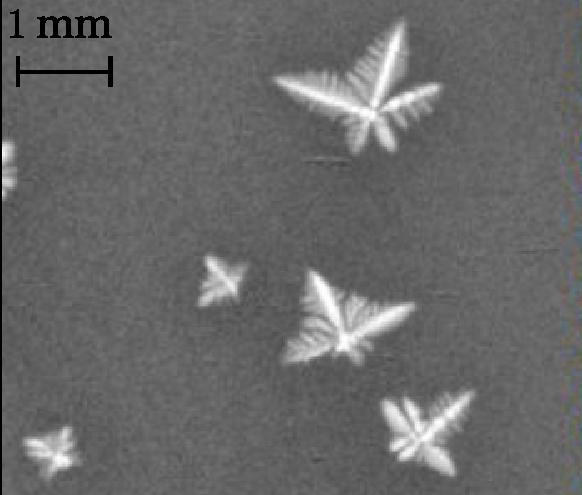
\includegraphics[height=4cm]{Chapter1/Graphics/dendrite_E.pdf}
	\caption{}
    \label{fig:dendrite_E}
  \end{subfigure}
\caption{In situ observation by X-ray radiography of the (a) columnar microstructure for \bin{Al}{4}{Cu} alloy \citep{buffet_measurement_2010}
and (b) equiaxed microstructure during solidification of \bin{Al}{10}{Cu} alloy \citep{bogno_growth_2013}.}
\label{fig:dendritic_growth}
\end{figure}
%
%-------------------------------------------------------------------------------------------------------------------------------------------------
%
%***********************************************
\subsection{Mush permeability}
%***********************************************
The dendritic geometry is crucial in solidification theory as it exhibits lower solid fraction compared to a microstructure formed by planar growth.
This fact has consequences on the fluid-structure interaction in the mushy zone, namely the liquid flow through dendrites. At the chill surface,
the solid  grows gradually from dispersed growing nuclei to a permeable solid skeleton, until finally grains have fully grown at the end of phase change.
In the intermediate state, the liquid flow in and out of the mushy zone through the dendrites is a key phenomenon from a rheological perspective.
%By defining a \emph{coherency temperature} $\Tcoh$, one can distinguish two behaviors. 
%For temperatures below $\Tcoh$ (usually at low solid fractions), the liquid flow is characterized by an intrinsic velocity. 
%As for temperature above $\Tcoh$,
%For the rest of this section, we will focus on the first behavior where liquid has a relative freedom to move inside the mushy zone.
The flow through the solid skeleton is damped by primary and secondary dendrites, resulting in momentum dissipation just like in saturated porous media. 
The famous \citet{darcy_les_1856} law relates the pressure gradient ($\nabvec p$) to the fluid velocity $\vec{v}$ (assuming a the solid phase is fixed), 
through the following equation \citep{rappaz_numerical_2003}:
%----------------------
\begin{align}
\label{eq:darcy}
& \vec{v} = \frac{\K}{\mul} \nabvec p
\end{align}
%----------------------
where $\mul$ is the liquid dynamic viscosity and $\K$ is the permeability tensor. The latter parameter has been the subject of numerous studies that aimed
to predict it from various microstructural or morphological parameters.
Some of these studies have started even before the first attempts to model macrosegregation by 
\citet{flemings_macrosegregation:_1967, flemings_macrosegregation:_1968-1,flemings_macrosegregation:_1968}. 
Basically, all models include the solid fraction, $\gs$, as input to predict mush permeability along with empirical data. 
An instance of such models is the work of \citet{xu_gravity-_1991}.
Some models rely additionally on the primary dendrite arm spacing $\pdas$ like Blake-Kozeny \citep{ramirez_evaluation_2003}, or the secondary 
dendrite arm spacing $\sdas$ like Carman-Kozeny, as a meaningful parameter to determine an isotropic permeability. 
Other models like \citet{poirier_permeability_1987,felicelli_simulation_1991} derive an anisotropic permeability based on both $\pdas$ and $\sdas$.

The present work uses Carman-Kozeny as a constitutive model for the isotropic permeability scalar (zero order tensor):
%----------------------
\begin{align}
\label{eq:permeability}
& \K  = \frac{\sdas^2 \gl^3}{180\brac{1-\gl}^2}
\end{align}
%-----------------------------------
%
%***********************************************
%
\section{Macrosegregation}
%
Macrosegregation generally stems from a solubility difference between a liquid phase and one or more solid phases, along with
a relative velocity between these phases. While the former is responsible for local solute enrichment or depletion, the latter
will propagate the composition heterogeneity on a scale much larger than just a few dendrites.
% http://dictionary.cambridge.org/grammar/british-grammar/little-a-little-few-a-few
This is why macrosegregation could be observed on the scale of a casting, up to several meters in length. 
While microsegregation can be healed by heat treatments, the alloy to speed up the diffusion process and allow homogenization, heterogeneities 
spanning on larger distances cannot be treated after solidification. It is obvious that macrosegregation is an irreversible defect. 
Failure to prevent it, may lead to a substantial decline in the alloy's mechanical behaviour and its serviceability.
Experimental investigations of macrosegregation in steels were the subject of numerous studies in the past, 
like the work of \citet{suzuki_mechanism_1973,shah_effect_1989,lesoult_macrosegregation_2005}. They were mainly motivated
by industrial research that aimed at reducing defective production caused by macrosegregation.
However, steel was not the only alloy that was investigated, probably because of its high melting point. 
Instead, many studies in the past relied on other metallic alloys as a replacement recourse, for their low
melting points, also for their well-known thermophysical and mechanical properties, such as aluminium-based alloys 
(aluminium-copper or aluminium-silicon) \citep{lesoult_equi-axed_2001,ferreira_macrosegregation_2004,ferreira_modeling_2009} and lead-tin/tin-lead alloys\citep{hebditch_observations_1974,prescott_convective_1994,hachani_experimental_2012}. Investigating macrosegregation 
was not only limited to metallic alloys, but also to organic compounds like the well-known 
sodium chloride \citep{wanqi_formation_1989}.
%--------------------------------------------------------
%
%
%\subsection{Causes}

Four main factors can (simultaneously) cause fluid flow leading to macrosegregation:
thermosolutal convection in the liquid, solidification and thermal shrinkage,
movement and sedimentation of equiaxed crystals and finally solid deformation.
%
\subsection{Liquid thermosolutal convection}
During solidification, the liquid density undergoes changes due to temperature gradients.
Generally for steels, an increasing temperature results in a lighter liquid phase and vice-versa.
These variations create a driving force of thermal convection in the melt, during which 
chemical species are redistributed by convective transport. While a uniform composition
is usually maintained throughout the liquid phase, solute gradients may appear in zones where
thermal convection currents are not sufficient to homogenise the liquid solution. 
Similarly to thermal gradient, a solute gradient is behind liquid density variations.
Nevertheless, the relationship between the liquid's composition and its density is a characteristic
of the alloy. While for some alloys, a positive solute gradient creates a positive density gradient,
for others the opposite is true, due to a heavier solute. Whether convection is solute or temperature
dominated, convection currents are important in the formation of macrosegregation, especially that 
phase densities vary considerably upon cooling the superheated alloy to room temperature.
%--------------
%\begin{subequations}
%\begin{align}
%\label{eq:rholiq}
%& \rhol = \rholref ( 1 - \betaT (T - \Tref) - \sum_{i} \betawil (\wil - \wilref) )  \\ 
%\label{eq:gradrholiq}
%& \nabvec\rhol = -\rholref (  \betaT \nabvec T + \sum_{i} \betawil \nabvec\wil  )
%\end{align}
%\end{subequations}
%--------------
%
%In \cref{eq:rholiq}, density is assumed to vary linearly with temperature and phase composition 
%for each chemical species (index $i$). The slopes defining such variations are respectively the 
%thermal expansion coefficient $\betaT$ and the solutal expansion coefficients $\betawil$, given by:
% \citep{kohler_peritectic_2008}
%
%--------------
%\begin{subequations}
%\begin{align}
%\label{eq:betaT}
%& \betaT =  -\frac{1}{\rholref} \brac{\frac{\partial\rhol}{\partial T}}  \\ 
%\label{eq:betawil}
%& \betawil = -\frac{1}{\rholref} \brac{\frac{\partial \rhol}{\partial \wil}}  
%\end{align}
%\end{subequations}
%--------------
%
%The linear fit assumes also that the density takes a reference value, $\rholref$, when temperature 
%and liquid composition reach reference values, respectively $\Tref$ and $\wilref$, while the
%coefficients $\betawil$ remain constant. However, in some 
%situations, a suitable thermodynamic database providing accurate density values is far better than a 
%linear fit, especially in the current context of macrosegregation. 
% Such possibility will be discussed later in the manuscript. %(cf. SECTION \red{TODO})\\ %TODO ) 
%In the presence of gravity, the density gradient in \cref{eq:gradrholiq}, causes thermosolutal convection 
%in the liquid bulk and a subsequent macrosegregation.
%
% 
\subsection{Solidification shrinkage}
Solid alloys generally have a greater density than the liquid phase ($\rhos > \rhol$), 
thus occupy less volume, with the exception of silicon where the opposite is true. 
Upon solidification, the liquid moves towards the solidification front to compensate for the volume 
difference caused by the phase change, as well as the thermal contraction. When macrosegregation is 
triggered by solidification shrinkage, we speak of \emph{inverse segregation}: while one would naturally expect 
negative macrosegregation near the contact with the chill, shrinkage-induced flow 
promotes the opposite phenomenon, by bringing solute-richer liquid towards the solidifying areas, thus raising 
their solute content, and resulting in a positively segregated solid.
In contrast to liquid convection, shrinkage flow may cause macrosegregation even without gravity.
%
%
\subsection{Movement of equiaxed grains}
%
%read pickering2013: http://www.msm.cam.ac.uk/phase-trans/2013/macro.pdf
Globular and equiaxed dendritic grains nucleate and grow in the liquid bulk where thermal gradients 
are weak, or in the presence of inoculants. Consequently, they are transported by the flow, thus floating 
or sedimenting depending on their density \citep{beckermann_modelling_2002}. During their movement, the nearby 
liquid is driven away before the grains finally settle in the end of solidification. Since solute-rich liquid
is expelled, a negative macrosegregation zone (often referred to as \emph{negative segregation cone} in cast ingots) 
is detected in their final position.
%
%
\subsection{Solid deformation} 
%
Stresses of thermal and mechanical nature are always found in casting processes 
(e.g. bulging between rolls in continuous casting). 
Deformation of the semi-solid in the mushy zone causes a relative solid-liquid 
flow in the inward (tensile stresses) or outward (compressive stresses) direction, causing macrosegregation.
%
\section{Other defects}
%
Apart from macrosegregation, other defects are also encountered in industrial processes. 
In the casting industry, defects like pores and cracks can be disastrous causing the cast product 
to be rejected. If possible, the product is reheated, remelted and then cast again. Otherwise it is scrapped.
From an economic point view, these operations are very expensive.
%
%-----------------
\begin{figure}[htbp]
\centering
   %------------
  \begin{subfigure}[t]{0.3\textwidth}
    \centering
	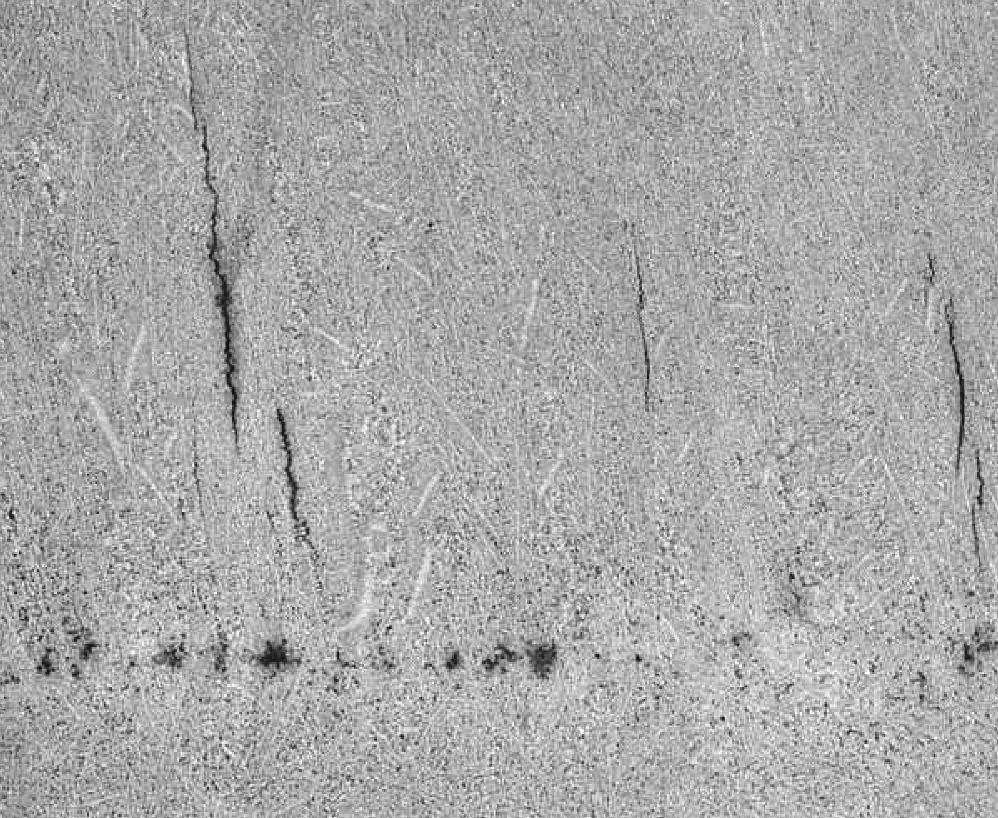
\includegraphics[height=3.5cm]{Chapter1/Graphics/cracks.png}
	\caption{}
    \label{fig:crack}
  \end{subfigure}
   %------------
   %\hspace{1cm}
   \begin{subfigure}[t]{0.35\textwidth}
    \centering
	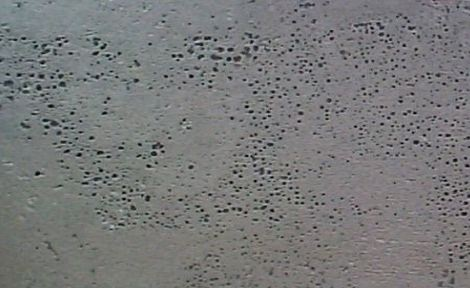
\includegraphics[height=3.5cm]{Chapter1/Graphics/porosity5.jpg}
	\caption{}
    \label{fig:porosity}
  \end{subfigure}
     %------------
   %\hspace{1cm}
   \begin{subfigure}[t]{0.3\textwidth}
    \centering
	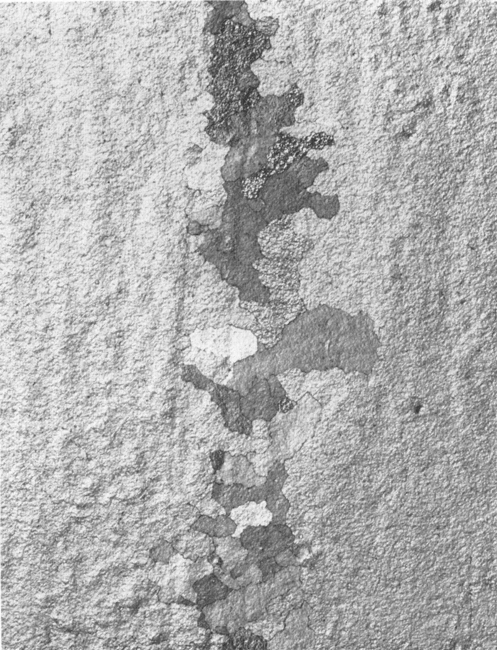
\includegraphics[height=3.5cm]{Chapter1/Graphics/freckle4.png} 
	\caption{}
    \label{fig:freckle}
  \end{subfigure}
\caption{Three instances of solidification-related defects found in cast products: 
(a) internal crack in continuous casting [Arcelormittal] (b) surface cavities in ingot casting \citep{carlson_modeling_2002}  
and (c) freckle in the form of a chain of equiaxed crystals in Ni-base superalloy investment casting \citep{giamei_nature_1970}.}
\label{fig:casting}
\end{figure}
%
%-----------------------------
%
\subsection*{Hot tearing} 
%
Hot tearing, also denoted solidification cracking or hot cracking, occurs in the mushy zone 
at high solid fractions when a failure or crack appears at vulnerable locations known as the \emph{hot spots}. 
They refer to liquid regions enclosed in the solid, where feeding stops, 
thus creating preferential sites for crack initiation and propagation, as in \cref{fig:crack}. 
The temperature range in which the steel is vulnerable to hot tearing is known as the brittleness 
temperature range (BTR). It corresponds to solid fractions greater than \num{90}\%.
Many factors can initiate the failure, but the main origin is a 
lack of liquid feeding required to compensate for the solidification shrinkage, while the mushy region
is exposed to tensile stresses arising from thermal gradients or due to an applied mechanical force.
%\begin{figureth}
% hottearing1: JM drezet, GDR 2013 Lausanne, contraintes residuelles.
% textwidth 
%{0.4}
%path 
%{Chapter1/Graphics/hottearing1.png}
% caption
%{Crack in an aluminium slab}
% label
%\label{fig:hottearing}
%\end{figureth}
%-------------------------------------------------------------------------------------------------------------------------------------------------
\subsection*{Porosity}
%reference: \url{http://www.afsinc.org/about/content.cfm?ItemNumber=6933} \\
%reference: \url{http://en.wikipedia.org/wiki/Casting_defect} \\
%
Porosity is a void defect formed inside the casting or at the outer surface. It may be attributed to two different factors.
Firstly, we speak of \emph{shrinkage porosity}, when a void forms as a result of density 
differences between the liquid and its surrounding dendritic solid network, the latter being generally denser 
than the former. After solidification is complete, the casting surface may look like \cref{fig:porosity}.
The second factor is the presence of dissolved gaseous phases in the melt. 
According to \citet{dantzig_solidification_2009}, these gases may be initially in the melt, or created by the 
reaction between the metal and water found in the air or trapped in grooves at the moulds surface. Providing sufficient cooling
and pressure drop in the liquid, the latter becomes supersaturated. 
The nucleation of a gaseous phase is then triggered.
%(just like when a cold bottle of coca-cola is opened !).
%
%-----------------
%\begin{figure}[htbp]
%Porosity1-2: http://www.afsinc.org/about/content.cfm?ItemNumber=6933
%Porosity3: http://www.weldreality.com/aluminumalloys.htm
%Porosity4: http://www.esab.com/global/en/education/new-lean-duplex-steels.cfm
%\centering
   %------------
  %\begin{subfigure}[t]{0.3\textwidth}
   % \centering
	%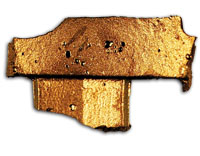
\includegraphics[width=\textwidth]{Chapter1/Graphics/porosity1.jpg}
	%\caption{Gas porosity in casting \citep{afs_american_2014}.}
    %\label{fig:porosity1}
  %\end{subfigure}
   %------------
  % \hspace{1cm}
   %\begin{subfigure}[t]{0.25\textwidth}
    %\centering
	%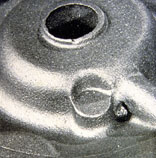
\includegraphics[width=\textwidth]{Chapter1/Graphics/porosity2.jpg}
	%\caption{Shrinkage porosity \citep{afs_american_2014}.}
    %\label{fig:porosity2}
  %\end{subfigure}
  %------------------------------
  %\vskip\baselineskip
  %------------------------------
  %\begin{subfigure}[t]{0.3\textwidth}
   % \centering
%	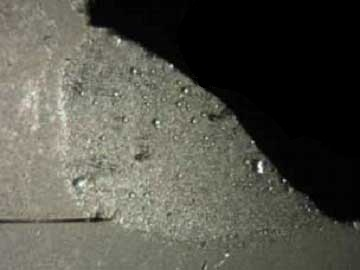
\includegraphics[width=\textwidth]{Chapter1/Graphics/porosity3.jpg}
%	\caption{Gas porosity in aluminium welding \citep{weldreality_aluminum_2014}.}
 %   \label{fig:porosity3}
  %\end{subfigure}
   %------------
 % \hspace{1cm}
 %  \begin{subfigure}[t]{0.25\textwidth}
 %   \centering
%	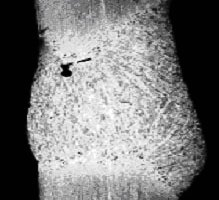
\includegraphics[width=\textwidth]{Chapter1/Graphics/porosity4.jpg}
%	\caption{Xray of volume void inside welded duplex steel \citep{esab_new_2014}.}
 %   \label{fig:porosity4}
 % \end{subfigure}
   %------------
%\caption{Examples of porosity in casting and welding} 
%\label{fig:porosity}
%\end{figure}
%
%-------------------------------------------------------------------------------------------------------------------------------------------------
%
\subsection*{Freckles or segregated channels} 
%
The origin of this defect, shown in \cref{fig:freckle}, is a combined effet of microsegregation and buoyancy forces. 
Upon solidification, solid forms while exchanging solutes with the liquid due to partitioning.
%(steels have a partition coefficient less than unity).
For a solute species that preferentially segregates into the liquid (partition coefficient less than unity)
and locally reduce the liquid density, a solutal driving force is created inside the mushy zone, generating convection currents, 
with "plume" shapes as often reported in the literature \citep{sarazin_studies_1992, schneider_modeling_1997,
saad_simulation_2015}. Temperature gradient is often an additional force of convection as the liquid density depends also temperature-dependent, 
the resulting driving force is then qualified as "thermosolutal".
%-------------------------------------------------------------------------------------------------------------------------------------------------
%
%
%\subsection{Investment casting}
%
% This process is widely used to cast single-crystal (SC) alloys for turbines and other applications 
% that require excellent mechanical behavior \citep{giamei_nature_1970}.
% When performed by directional solidification, thermosolutal forces thrust segregated species outside of the 
% mushy zone into the liquid bulk. The segregation scale ranges from a few dendrites to a few hundreds 
% of them, hence forming "long and narrow trails" (\cref{fig:freckle1}) as described by \citet{felicelli_simulation_1991}. 
% Freckles are frequently formed by small equiaxed grains (\cref{fig:freckle2}), probably caused by a uniform temperature gradient 
% that settles as the channels become richer in solute. They can be observed on the ingot's surface, as well as in the volume.
%------------
% \begin{figure}[htbp]
%freckle1: http://user.engineering.uiowa.edu/~becker/solcast.html
%freckle2: beckermann 2002 or Giamei ?
%freckle3: Giamei 
% \centering
   %------------
  % \begin{subfigure}[t]{0.25\textwidth}
    % \centering
	% 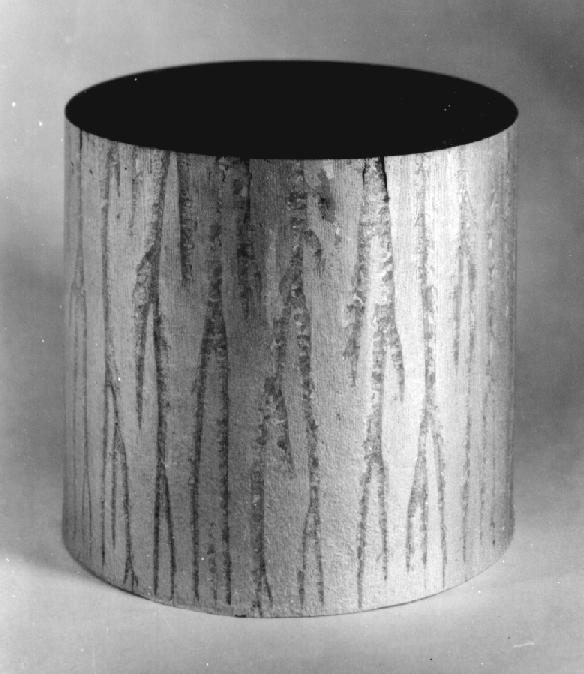
\includegraphics[height=5cm]{Chapter1/Graphics/freckle1.png}
	% \caption{Small cylinder ingot showing freckles on the outer surface}
    % \label{fig:freckle1}
  % \end{subfigure}
   %------------
   % \qquad %\hspace{2cm}
   % \begin{subfigure}[t]{0.25\textwidth}
    % \centering
	% 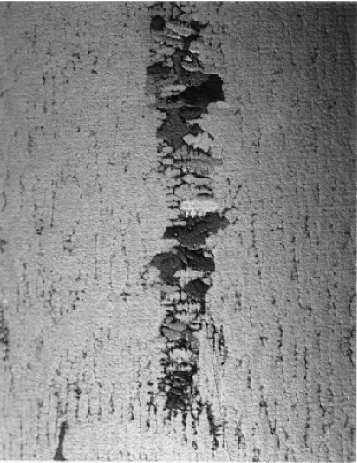
\includegraphics[height=5cm]{Chapter1/Graphics/freckle2.png}
	% \caption{Zoomed image showing the microstructure in one freckle}
    % \label{fig:freckle2}
  % \end{subfigure}
   %------------
% \caption{Freckles in directional casting of nickel-base superalloys} 
% \label{fig:freckle}
% \end{figure}
%--------------------------------------------------------
%
%*********************************
\section{Industrial Worries}
%*********************************
Steel production has continuously increased over the years to meet the industrial needs. \Cref{fig:steel_production} shows this increase between 1980 and 2013 with a 
clear dominance of the Chinese production. Quality constraints have also increased where specific grades of steel are needed in critical applications such as mega-structures
in construction and  heavy machinery. Therefore, alloys with defects are considered vulnerable and should be avoided as much as possible during the casting process. As such, steelmakers have been investing
in research, with the aim of understanding better the phenomena leading to casting problems, and improve the processes when possible.
\begin{figure}[htbp]
\centering
\begin{tikzpicture}
 \pgfkeys{%
    /pgf/number format/set thousands separator = {}}
\begin{axis}
[
	table/col sep=comma,
	smooth, %ybar
	stack plots=y,
	area style,
	enlarge x limits=false,
	legend pos=north west,
	scaled ticks=true,
	xlabel=Year,
	ylabel=Production (tons),
	xticklabel style={/pgf/number format/fixed},
	xtick={1980,1990,2000,2010},
	%x tick label style={rotate=45,anchor=east},
	%width=0.5\textwidth
]
\addplot table [x=Year, y expr=\thisrow{EU}*1000] {Chapter1/Data/steel_production.csv} \closedcycle ;
%\addlegendentry{EU (27)}
\addplot table [x=Year, y expr=\thisrow{China}*1000] {Chapter1/Data/steel_production.csv}\closedcycle;
%\addlegendentry{China}
\addplot table [x=Year, y expr=\thisrow{World}*1000] {Chapter1/Data/steel_production.csv}\closedcycle;
%\addlegendentry{World}
\legend{EU (27), China, World}
\end{axis}
%\addplot table [x expr=\coordindex, y=EU] {Chapter1/Data/steel_production.csv};
\end{tikzpicture}
\caption{Evolution curves of crude steel worldwide production from 1980 to 2013 \citep{wsa_world_2014}.}
\label{fig:steel_production}
\end{figure}

Simulation software dedicated to alloy casting is one of the main research investments undertaken by steelmakers. 
These tools coming from academic research
are actively used to optimize the process. 
However, few are the tools that take into account the casting environment. 
For instance, the continuous casting process, in
\cref{fig:casting}, is a chain process where the last steps involve rolls, water sprays and other components. 
A dedicated software is one that can provide the geometric requirements with suitable meshing capabilities, 
as well as respond to metallurgical and mechanical requirements, mainly by handling:
%
\begin{itemize}
\itemsep0em
\item moulds and their interaction with the alloy (thermal resistances ...)
\item alloy filling and predicting velocity in the liquid and mushy zone
\item thermomechanical stresses in the solid
\item multicomponent alloys and predicting macrosegregation
\item microstructure and phases
\item finite solute diffusion in solid phases
\item real alloy properties (not just constant thermophysical/thermomechanical properties)
\end{itemize}
%
%
%*********************************
\section{Project context and objectives}
%*********************************
%
%*********************************s
\subsection{Context}
%*********************************
The European Space Agency (ESA) has been actively committed, since its foundation in 1975, in the research field.
Its covers not only exclusive space applications, but also fundamental science like solidification. 
This thesis takes part in the ESA project entitled \ccemlcc, abbreviating
"\textbf{C}hill \textbf{C}ooling for the \textbf{E}lectro-\textbf{M}agnetic \textbf{L}evitator in relation with 
\textbf{C}ontinuous \textbf{C}asting of steel".
The three-year contract from 2011 to late 2014 denoted \ccemlcc II, was preceded by an initial project phase, \ccemlcc I,
from 2007 to 2009. The main focus is studying containerless solidification of steel under microgravity conditions. 
A chill plate is used to extract heat from the alloy, simulating the contact effect with a mould in continuous casting
or ingot casting.
A partnership of 7 industrial and academic entities was formed in \ccemlcc II. 
Here is a brief summary of each partner's commitment:\\

\textbf{Academic partners} 
 \begin{itemize}
\itemsep0em
\item Center for Material Forming (CEMEF) - France: numerical modelling of microgravity chill cooling experiments
\item Deutsches Zentrum für Luft- und Raumfahrt (DLR or German Aerospace Centre) and Ruhr Universität Bochum (RUB) university - Germany:  preparation of a chill cooling device 
for electromagnetic levitation (EML), microgravity testing and investigation of growth kinetics 
in chill-cooled and undercooled steel alloys
\item University of Alberta - Canada: impulse atomization and spray deposition of the D2 tool steel 
\item University of Bremen - Institut für Werkstofftechnik (IWT) institute - Germany: 
study of D2 tool steel melt solidification in atomization processing
\end{itemize}

\textbf{Industrial partners}
\begin{itemize}
\itemsep0em
\item ARCELORMITTAL (France): elaboration of a series of steel grades used in microgravity and ground-based studies
\item METSO Minerals Inc.  (Finland): material production with D2 tool steel for spray forming
\item TRANSVALOR (France): development and marketing of the casting simulation software \thercast
\end{itemize}

CEMEF, as an academic partner, contributed to the work by proposing numerical models in view of predicting the chill cooling of steel droplets. 
A first model was developed by \citet{rivaux_simulation_2011}. 
The experimental work by DLR considered various facilities and environments to set a droplet of molten alloy in levitation: 
EML (\cref{fig:eml}) for ground-based experiments, 
microgravity during parabolic flight or sounding rockets and last, microgravity condition on-board the International Space Station (ISS).
%---------
\begin{figureth}
% textwidth 
{0.5}
%path 
{Chapter1/Graphics/eml1.jpg}
% caption
{Electromagnetic levitation \citep{dlr_electomagnetic_2014}.}
% label
\label{fig:eml}
\end{figureth}
%-------------------------------------------------------------------------------------------------------------------------------------------------
%
%%*********************************
\subsection{Ojectives and outline}
%*********************************
The main focus of the present thesis is predicting macrosegregation with liquid dynamics assuming a fixed solid phase, i.e. no account of solid 
transport (e.g. equiaxed crystals sedimentation) and no account of solid deformation. At CEMEF, this scope has been adopted in previous 
studies by \citet{gouttebroze_modelisation_2005, liu_finite_2005, mosbah_multiple_2008, rivaux_simulation_2011, carozzani_developpement_2012}.
Nevertheless, many modelling features evolved with time such as going from two-dimensional to three-dimensional modelling, resolution schemes
for each of the conservation equations: energy, chemical species and liquid momentum, Eulerian or Lagrangian descriptions, 
modelling of grain structure and others. In this thesis, we propose a numerical model that takes into account 
i) the energy conservation in a temperature formulation based on a thermodynamic database mapping,
ii) the liquid momentum conservation with thermosolutal convection and solidification shrinkage as driving forces, 
iii) solute mass conservation with solidification shrinkage (to predict inverse segregation) and 
iv) solidification paths at full equilibrium for multicomponent alloys. 
Moreover, all equations are formulated in a pure Eulerian description while using the level set method to keep 
implicitly track of the interface between the alloy and the surrounding gas. 

To the author's knowledge, this work 
combining macrosegregation prediction using the level set methodology to track the metal-air interface during 
shrinkage has no precedent in casting and solidification literature. The model couples in a weak fashion, all four
conservation equations presented in \cref{fig:mindmap}, showing on the one hand, that microsegregation is an essential 
common link between these equations, while on the other hand, the level set interacts with conservations equations by
giving the interface position. 
%
\subsubsection{Numerical tools}
The current thesis developments are done using C++ language as a part of the
in-house code, known as \cimlib \citep{mesri_advanced_2009}. It's a finite element library with an object-oriented hierarchy
consisting of global finite element solvers for physical differential equations, also point-wise and element-wise solvers for 
preprocessing and postprocessing the finite element solution. It is also highly parallelised with MPICH2, which makes it possible
to handle large meshes with heavy operations like mesh partitioning and adaptation. Side utilities for plotting and analysis
are also developed, using python language.

\subsubsection{Content outline}
This manuscript consists of 5 chapters. In \textbf{chapter 2}, a short review introduces the state-of-art in the literature of 
macroscopic modelling of solidification with transport of energy, species, mass and momentum. \textbf{Chapter 3} provides details
of the energy conservation equation then introduces a new temperature-based solver compatible with thermodynamic databases
% to predict, at equilibrium, variable solidification paths during macrosegregation.
\textbf{Chapter 4} focuses on the mass and momentum conservation equations 
and their derivation in the context of a single metallic domain (i.e. without 
the level set method) where the solid is assumed a fixed and rigid body. As an 
application, this chapter shows a breakthrough comparison between purely macroscopic 
and mesoscopic-macroscopic approaches in predicting the hydrodynamic instabilities 
that lead to channel segregation.
The derived energy, mass and momentum equations for the monodomain model are revisited 
in \textbf{chapter 5} in the context of the level set method to predict solidification shrinkage.
The influence of shrinkage on macrosegregation is then studied in two different applications.

\begin{figureth}
% textwidth 
{1.0}
%path 
{Chapter1/Graphics/mindmap.pdf}
% caption
{A graphical representation of the main elements of the numerical approach, 
for a macrosegregation model with the level set methodology, when no solid deformation or movement are considered. 
The dashed lines represent the possible interaction between the components.}
% label
\label{fig:mindmap}
\end{figureth}
%--------------------------------------------------------
%\subsection*{Biblio test}
%\citet{carozzani_direct_2013} is textual \\
%\citep{carozzani_direct_2013} is parenthetical \\
%--------------------------------------------------------
%\subsection*{Cross reference test}
%ref gives \ref{eq:betaT} \\
%cref gives \cref{eq:betaT} \\
%Cref gives \Cref{eq:betaT} \\
%autoref gives \autoref{eq:betaT} \\

%ref gives \ref{fig:porosity1} \\
%cref gives \cref{fig:porosity1} \\
%Cref gives \Cref{fig:porosity1} \\
%autoref gives \autoref{fig:porosity1} \\


%\section*{Trying \emph{SIUNITX}}
%Here i wana test the SI units package via the commands \num{.3e45} and the unit \si{\kilo\metre}
%then i wanted to see if we combine both via \SI{.3e45}{\kilo\metre} then finally my personal command
%\SI{231e-4}{\uacceleration} \\
%\SI{231e-4}{\ucomposition} C \\
%\SI{231e-4}{\uvelocity} \\
%\SI{231e-4}{\uconductivity} \\
%\SI{231e-4}{\umasscapacity} \\
%\SI{231e-4}{\uvolumecapacity} \\
%Will it work \num{.3e45}   ,  \num{3.45d-4}   , \numlist{10;30;50;70} ,  \numrange{10}{30}